\section{Gemessene Unvollständigkeit von RS-B2-CPS und Pyro(J)}

Wie in Kapitel 3 gesehen, wurde die Unvollständigkeit von \cite{bachelor}  mit Hilfe einer sternförmigen Anfrage nachgewiesen. Diese Ergebnisse sollten reproduziert werden. Da diese Ergebnisse so nicht reproduzierbar waren, wird ein Erklärungsansatz vorgeschlagen.

\subsection{Prüfung der Ergebnisse aus Kapitel 3}
Es wurden zwei Tests durchgeführt. Hierzu wurden zwei sternförmige Anfragen erzeugt. Jede Anfrage wurde ausgeführt und die Anzahl der unterschiedlichen Pläne gemessen.

\begin{figure}[h]
\centering

\begin{tabular}{|l|l|l|}
\hline
Relationen & RS-B2 & RS-B1 \\ \hline
5          & 384       & 384       \\ \hline
7          & 46080     & 46080     \\ \hline
\end{tabular}





\caption{Anzahl Pläne nach Regelmenge und Anzahl-Relationen}
\label{protoUnvollstaendig}
\endfigure

Im Gegensatz zu \cite{bachelor} konnte nicht festgestellt werden, dass RS-B2 schlechter als die Vergleichsregelmenge RS-B1 funktioniert.


\subsection{Erklärungsansatz: Pyros Expansionsalgorithmus}

Der Grund für die Abweichung mag am Expansionsalgorithmus in Pyro liegen. Der verwendete Expansionsalgorithmus (vgl. Abb. \ref{ExpandDAG}) ist vollständig für die Regelmenge RS-B1. Ob dies auch für die Regelmenge RS-B2 zutrifft, wird im Folgenden an einem konkreten Beispiel geprüft.

\begin{figure}[ht]
  \centering
  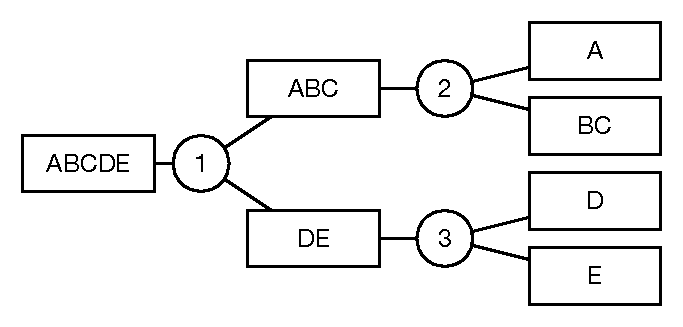
\includegraphics[scale=0.75]{05_ResultsEvaluation/00_media/PyroInital_0.pdf}
  \caption{Initialer Query Tree}
  \label{PyroInital}
\end{figure}

\begin{figure}[ht]
  \centering
  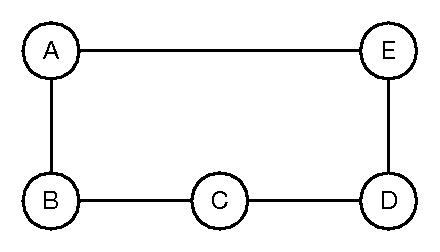
\includegraphics[scale=0.75]{05_ResultsEvaluation/00_media/PyroJoinGraph.pdf}
  \caption{Join-Graph}
  \label{PyroJoinGraph}
\end{figure}

Die Prüfung des Algorithmus erfolgt in vereinfachter Form am Beispiel des in Abb. \ref{PyroInital} dargestellten Query-Tree und Join-Graphen aus Abb. \ref{PyroJoinGraph}. Um die Darstellung zu vereinfachen, wird die Regel Kommutativität der Regelmenge nicht angewendet. Es bleiben also linke-Assoziativität, rechte-Assoziativität und Exchange erhalten.

In einem ersten Schritt sollen die Regeln auf Planknoten 1 angewendet werden. Da die untergeordneten Planknoten noch nicht expandiert wurden, muss die Expansion auf die Knoten 2 bzw. 3 angewendet werden. Da sich auf Knoten 3 keine Regel anwenden lässt, wird dieser Knoten als expandiert markiert. Auf den Knoten 2 kann Assoziativität angewendet werden. Es entsteht so der neue Knoten 4. Auf Knoten 4 lässt sich keine Regel anwenden. Alle Regeln wurden für Knoten 2 angewendet, daher kann Knoten 2 als expandiert markiert werden.

Da nun alle untergeordneten Knoten expandiert sind, können auf der Ebene von Knoten 1 alle Regeln angewendet werden. Hier ist die Anwendung von Exchange am interessantesten. Es werden die neuen Knoten 7, 8, 9, 10, 11 geschaffen. Da auf die Knoten 7, 9 keine weiteren Regeln angewendet werden dürfen, bricht der Algorithmus ab. 

\begin{figure}[ht]
  \centering
  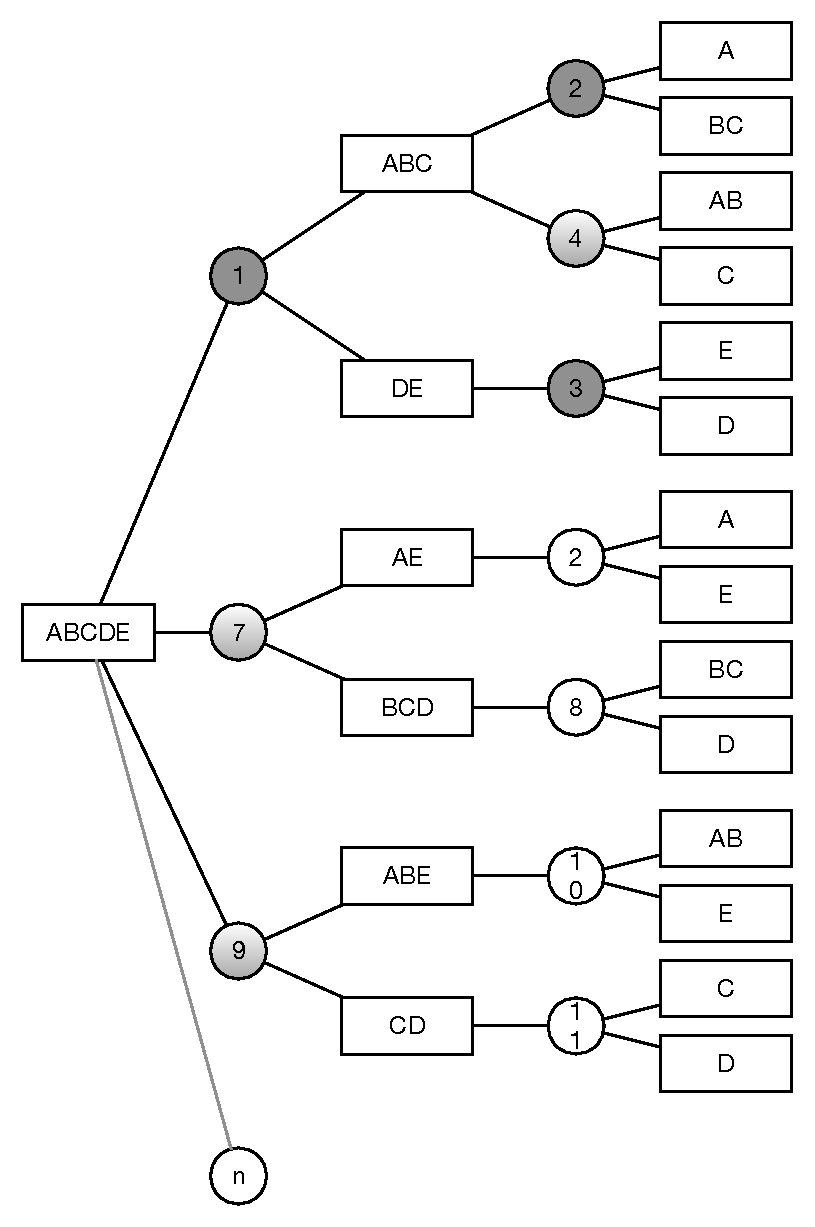
\includegraphics[scale=0.75]{05_ResultsEvaluation/00_media/PyroResult.pdf}
  \caption{Expandierter Query Tree}
  \label{ExpandedQueryTree}
\end{figure}

Wie in Abb. \ref{ExpandedQueryTree} zu erkennen, sind die Regeln nicht auf alle Teilbäume angewendet worden. Der gesamte Suchraum wurde nicht erforscht. Einer der Unterschiede zwischen dem von Pyro verwendeten und dem in Abb. \ref{ExpandDAG} gezeigten Expander ist, dass sobald ein neuer Planknoten gefunden wurde versucht wird alle Regeln, solange es möglich ist auf den gesamten Teilbaum erneut anzuwenden. So werden auch neue, untergeordnete Teilbäume in die Expansion einbezogen und der gesamte Suchraum im konkreten Beispiel erforscht.


\subsection{Prüfung der theoretischen Unvollständigkeit}
In Kapitel 3 wurde ein spezieller Fall vorgestellt, in dem die Unvollständigkeit der Regelmenge RS-B2 gezeigt wurde. Auch dieses Beispiel wurde geprüft.

Die Genaue Konfiguration kann entweder in Abbildung 3.1 bzw. Abbildung \ref{configUnvollstae} gefunden werden.

\begin{figure}[ht]
  \centering
  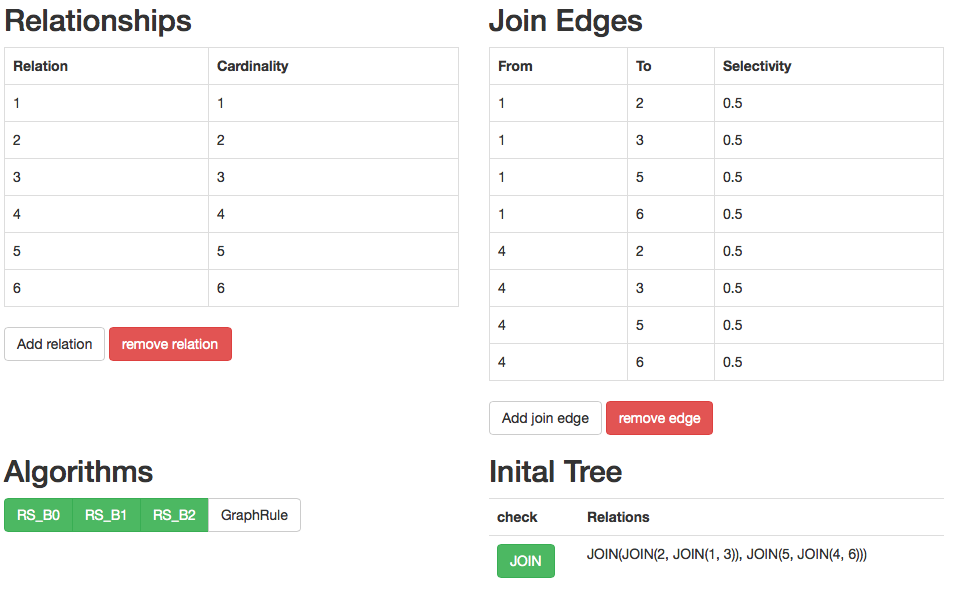
\includegraphics[width=\textwidth]{05_ResultsEvaluation/00_media/Vollstaendigkeitstest.png}
  \caption{Konfiguration: Vollständigkeitstest}
  \label{configUnvollstae}
\end{figure}

Bei den Tests zeigt sich (vgl. Abb. \ref{Result:Unvollstaendigkeit}), dass trotz der Wahl des akkuraten Transformatuonsenumerators korrekte Anzahl der Pläne mit RS-B2 nicht erreicht werden konnte. Die Menge der gefundenen Pläne liegt bei nur knapp 50\% der Pläne, die eigentlich zu erwarten sind. Auch die Anzahl der generierten Äquivalenzklassen ist stark reduziert. Durch diese Reduktion an Knoten konnte jedoch auch der Aufwand für die Enumeration um fast 50\% gesenkt werden.

\begin{figure}[ht]
\centering
\begin{tabular}{|l|l|l|l|}
\hline
                        & {\bf RS-B0} & {\bf RS-B1} & {\bf RS-B2} \\ \hline
{\bf Äuqivalenzklassen} & 101         & 101         & 85          \\ \hline
{\bf Pläne}             & 10.752      & 10.752      & 5.760       \\ \hline
{\bf Dauer (ms)}        & 2.764.217   & 2.620.888   & 1.378.230   \\ \hline
\end{tabular}
\caption{Resultat: Vollständigkeitstest}
  \label{Result:Unvollstaendigkeit}
\end{figure}

Die Unvollständigkeit der Regelmenge RS-B2 ist mit diesem Test erneut belegt. In der nächsten Sektion soll näher untersucht werden, in welchen Fällen die Regelmenge unvollständig ist.